% This file compiles with both LuaLaTeX and XeLaTeX
\documentclass[11pt]{article}

% Change "review" to "final" to generate the final (sometimes called camera-ready) version.
% Change to "preprint" to generate a non-anonymous version with page numbers.
\usepackage[review]{acl}
\usepackage{makecell}
% This is not strictly necessary, and may be commented out,
% but it will improve the layout of the manuscript,
% and will typically save some space.
% \usepackage{microtype}

% If the title and author information does not fit in the area allocated, uncomment the following
%
%\setlength\titlebox{<dim>}
%
% and set <dim> to something 5cm or larger.

% These font selection commands work with
% LuaLaTeX and XeLaTeX, but not pdfLaTeX.
\usepackage[english,bidi=default]{babel} % English as the main language.
\babelfont{rm}{TeXGyreTermesX} % similar to Times
%%% include whatever languages you need below this line
\babelprovide[import]{hindi}
\babelfont[*devanagari]{rm}{Lohit Devanagari}
\babelprovide[import]{arabic}
\babelfont[*arabic]{rm}{Noto Sans Arabic}


%\usepackage{polyglossia}
%\setdefaultlanguage{english}
%\setotherlanguages{arabic,russian,thai,hindi,kannada}
\usepackage{subcaption}
\usepackage{tikz}
\usepackage{linguex}
\usepackage{multicol}
\usepackage{amsmath, amssymb,stackengine,scalerel}
\usetikzlibrary{positioning}

%%%%%


\title{Does Representation Matter in Tonotactic Learning: Comparing String and Autosegmental Models}

% Author information can be set in various styles:
% For several authors from the same institution:
% \author{Author 1 \and ... \and Author n \\
%         Address line \\ ... \\ Address line}
% if the names do not fit well on one line use
%         Author 1 \\ {\bf Author 2} \\ ... \\ {\bf Author n} \\
% For authors from different institutions:
% \author{Author 1 \\ Address line \\  ... \\ Address line
%         \And  ... \And
%         Author n \\ Address line \\ ... \\ Address line}
% To start a seperate ``row'' of authors use \AND, as in
% \author{Author 1 \\ Address line \\  ... \\ Address line
%         \AND
%         Author 2 \\ Address line \\ ... \\ Address line \And
%         Author 3 \\ Address line \\ ... \\ Address line}

\author{First Author \\
  Affiliation / Address line 1 \\
  Affiliation / Address line 2 \\
  Affiliation / Address line 3 \\
  \texttt{email@domain} \\\And
  Second Author \\
  Affiliation / Address line 1 \\
  Affiliation / Address line 2 \\
  Affiliation / Address line 3 \\
  \texttt{email@domain} \\}

\begin{document}
\maketitle
\begin{abstract}

This paper investigates whether tonotactic learnability differs across 
representational choices. We conduct an experiment by using the same 
dataset but over two different representations: string and autosegmental 
representations (ARs). Two learning models are used: Maximum Entropy 
(MaxEnt) model and the Bottom-Up Factor Inference Algorithm (BUFIA), 
allowing us to examine whether differences in learning outcomes arise from 
the learning model as well as from the representation. Using identical 
training and testing datasets across conditions, we evaluate five 
implemented combinations: Baseline-Str, Baseline-AR, MaxEnt-Str, BUFIA-Str, 
and BUFIA-AR. The results show that (1) for the baseline grammar, which is 
static and surface-based, representational choice does not affect learning 
outcomes; and (2) for computationally learned grammars, performance is 
strongest when grammars are induced over ARs under a graph-based 
categorical learner. These findings suggest that representation plays an 
important role in tonotactics learning than probabilistic weighting 
mechanisms.
\end{abstract}

\section{Introduction}

This paper focuses on the learning of tonal phonotactics, or tonotactics, 
which address the question of the well-formedness of how tones and 
tone-bearing units (TBUs, such as syllable or mora) are organized in tonal 
languages. 

For a long time, tonotactics has not received the same level of research 
attention as segmental phonology, despite the widespread distribution of 
tone across the world’s languages \citep{yip2002tone}. One possible reason 
for this gap lies in representational differences. Segmental phonotactics is 
typically modeled using linear representations such as strings, which makes 
it readily compatible with a wide range of existing learning models. 
Tonotactics, by contrast, has long been analyzed over non-linear 
structures, most widely used autosegmental representations 
\citep{goldsmith1976autosegmental}. This representational challenge has 
contributed to a dearth of computational models that operate directly over 
non-linear tonal structure, with many approaches instead flattening tonal 
patterns into strings to accommodate linear learning frameworks. Although a 
substantial body of work has argued for the inadequacy of linear 
representations for capturing tonal generalizations 
\citep{clements2010autosegmental,oddenintroducing2013} and for 
computational learning 
\citep{jardine2016locality}, studies demonstrating clear advantages of 
non-linear representations over strings in tonotactics remain relatively 
limited.

In this paper, we address two questions: (1) how effectively tonotactics can 
be learned over ARs, and (2) whether ARs influence learning outcomes 
compared with alternative string-based representations. To address these 
questions, we encoded the same dataset in both string and AR formats to two 
versions of the Bottom-Up Factorial Inference Algorithm (BUFIA) 
\citep{chandleeBufia2019}: one operating over strings and the other directly 
over ARs \citep{li2025learning}. As a reference, a set of linguistically 
motivated grammars, also encoded over both string and AR, serves as a 
baseline for comparison. Additionally, we include a probabilistic learner, 
Maximum Entropy model \citep{hayes2008maximum}, to examine whether the 
absence of AR structure can be compensated for by probabilistic modeling. 
A cross-fold validation is conducted for comparing performance of models 
over varying representation. In two constructed test set, in addition to the 
positive data from the held-out set, matching size of negative forms 
are also added into the test sets to see if models overgeneralize. 

Admittedly, a more complete study should also include MaxEnt operating over 
ARs. However, the current implementation of MaxEnt does not support learning 
directly from graphs. Despite this limitation, this comparison still allows 
us to assess whether a structural representation will contribute to learning.

The results yield three main findings. First, representational choice does 
not affect outcomes when the grammar is a fixed, static set of constraints, 
provided that the two representations stand in a one-to-one correspondence. 
For computationally learned grammars, when the representation is changed, 
model performance improves, with BUFIA-AR emerging as the most robust model 
across conditions. This advantage is not compensated for by probabilistic 
modeling, which in fact has a below baseline performance.

Overall, this work highlights the importance of incorporating linguistically 
meaningful representations into computational models of phonological 
learning.

\section{Backgrounds}

This section outlines the theoretical background and computational methods 
for two representational choices: string and ARs. We adopt a model-theoretic 
perspective to describe these representations which treats them as distinct 
types of relational structures \citep{rogers2013,
	chandleeBufia2019, rogers.lambert2019mol}. From a modeling perspective, the difficulty 
of formally characterizing ARs is central to understanding the learning 
process.

\subsection{Linear vs.\ Non-linear Representations}

We define a phonological representation as relational structures of the 
form $\langle D, \mathcal{R} \rangle$, where $D$ is a finite domain of 
positions, and $\mathcal{R}$ is a set of relations that connects the 
composing units of the phonological representation. 

In a string representation, structure is single-tiered. The signature typically includes unary labeling relations indicating segmental or tonal identity and a single binary successor relation $\lhd$ defining linear order. For example, a string model of \textit{L.HL} is shown in Figure~\ref{sec2.fig.string}. The domain $D=\{1,2,3,4\}$ specifies four positions, labeled by tone and boundary symbols, and the successor relation encodes temporal sequencing. Structural dependencies must therefore be expressed indirectly through symbol combinations or longer contexts.

\begin{figure}[ht]
	\centering
		\begin{minipage}{0.6\linewidth}
	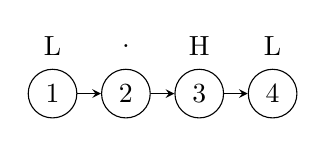
\begin{tikzpicture} [->, >=stealth, node distance=0.5cm,
		circleNode/.style={draw, circle, minimum size=0.2cm}]
		% Nodes
		\node[circleNode] (1) {1};
		\node[circleNode, right=0.3cm of 1] (2) {2};
		\node[circleNode, right=0.3cm of 2] (3) {3};
		\node[circleNode, right=.3cm of 3] (4) {4};
                \node[align=center,node distance=6mm] (l1) [above of = 1] {L};
                \node[align=center,node distance=6mm] (l2) [above of = 2] {.};
                \node[align=center,node distance=6mm] (l3) [above of = 3] {H};
                \node[align=center,node distance=6mm] (l4) [above of = 4] {L};
                \draw[->] (1) -- (2);
		\draw[->] (2) -- (3);
		\draw[->] (3) -- (4);
	\end{tikzpicture}
\end{minipage}
		\begin{minipage}{0.3\linewidth}
			\small
			\begin{align*}
				D &= \{1, 2, 3, 4\} \\
				L &= \{1,4\}\\
				H &=\{3\}\\
				. &= \{2\}\quad\\
				\lhd &= \{\langle1,2\rangle,\langle2,3\rangle,
				\langle3,4\rangle\}
			\end{align*}
		\end{minipage}
	
	\caption{String model when $\Sigma = \{H,L, .\}$ for \textit{HLH}}
	\label{sec2.fig.string} 
\end{figure}

ARs, in contrast, correspond to multi-tier relational structures. The signature includes multiple successor relations, each defined over a tier (e.g., tone, mora, syllable), as well as an association relation $\alpha$ linking elements across tiers. In this representation, structural dependencies such as tone spreading or contour formation are encoded directly as relations rather than inferred from symbol sequences.

\begin{figure}[ht]
	\centering
	\begin{minipage}{0.3\textwidth}
		\centering
		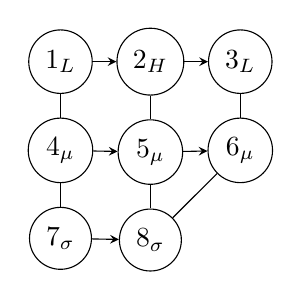
\begin{tikzpicture}[
			>=stealth,
			circleNode/.style={draw, circle},
			]
			% Tone tier
			\node[circleNode] (t1) {1$_L$};
			\node[circleNode, right=0.3cm of t1] (t2) {2$_H$};
			\node[circleNode, right=.3cm of t2] (t3) {3$_L$};
			
			% Mora tier
			\node[circleNode, below=.3cm of t1] (m1) {4$_\mu$};
			\node[circleNode, below=.3cm of t2] (m2) {5$_\mu$};
			\node[circleNode, below=.3cm of t3] (m3) {6$_\mu$};
			
			% Syllable tier
			\node[circleNode, below=.3cm of m1] (s1) {7$_\sigma$};
			\node[circleNode, below=.3cm of m2] (s2) {8$_\sigma$};
			
			% Association lines (alpha)
			\draw (t1) -- (m1);
			\draw (t2) -- (m2);
			\draw (t3) -- (m3);
			
			\draw (m1) -- (s1);
			\draw (m2) -- (s2);
			\draw (m3) -- (s2);
			
			% Successor relations (lhd)
			\draw[->] (t1) -- (t2);
			\draw[->] (t2) -- (t3);
			
			\draw[->] (m1) -- (m2);
			\draw[->] (m2) -- (m3);
			
			\draw[->] (s1) -- (s2);
			
		\end{tikzpicture}
	\end{minipage}
	\hfill
	\begin{minipage}[b]{0.3\textwidth}
		\small
		\begin{align*}
			D &= \{1, 2, 3, 4, 5, 6, 7, 8\} \\
			L &= \{1,3\}\quad H =\{2\}\quad \mu= \{4,5,6\}\quad  \sigma = \{7,8\} \\
			\lhd &= \{\langle1,2\rangle,\langle2,3\rangle,
			\langle4,5\rangle,\langle5,6\rangle,
			\langle7,8\rangle\} \\
			\alpha &= \{(1,4),(2,5),(3,6),
			(4,7),(5,8),(6,8)\}
		\end{align*}
	\end{minipage}
\caption{Autosegmental model when $\Sigma = {H,L,\sigma, \mu}$.}
\end{figure}

From a learning perspective, this distinction has important consequences. 
For strring representation, the 
encode cross-tier dependencies implicitly through alphabet expansion or increased contextual complexity, whereas ARs encode these dependencies explicitly in the relational structure. As a result, equivalent phonological generalizations may require more complex constraints in string models while remaining locally expressible in ARs. We therefore treat representational format not as a notational choice but as a factor shaping inductive bias.

This view leads to a concrete prediction: if structural information is directly available to the learner, grammars induced over ARs should achieve comparable or improved generalization using constraints of equal or lower complexity.

\subsection{Phonotactic Learning Models}

The main model used in this paper is based on two versions of the Bottom-Up 
Factor Inference Algorithm (BUFIA; \citet{chandleeBufia2019}). BUFIA is a 
categorical phonotactic learner that traverses a hypothesis space organized as 
a partially ordered set: all logically possible structures over a given 
alphabet are ordered by the containment (or sub/superfactor) relation. As 
illustrated in Figure [maybe???] for strings over the alphabet ${a,b}$, more 
general structures (e.g., the empty string or singletons) occupy lower 
positions in the space, while more specific structures appear higher. For any 
given structure, those that properly contain it are its \textit{superfactors} 
(positioned above), and those that it properly contains are its 
\textit{subfactors} (positioned below). For all its superfactors, only those 
one level above the current candidates are referred to as their ``next 
superfactors''

Two core operations of BUFIA determine its upward search or pruning: 
containment and the sub/superfactor relation. The learner is provided with a 
set of positive data and a user-defined complexity bound $k$. The search begins 
from an initial structure (typically the empty structure). For each candidate, 
BUFIA checks whether it is contained in the positive dataset. If it is 
attested, the learner generates its next superfactors and continues searching 
upward. Otherwise, the structure is identified as a forbidden factor (i.e., a 
constraint), and prune off its superfactors from space for not checking. In 
this way, BUFIA identifies the most general unattested structures and prunes 
all more specific structures that would necessarily also be forbidden. The 
resulting grammar guarantees full coverage of the observed data while remaining 
maximally general.

A key advantage of BUFIA is its representational flexibility. The algorithm 
operates over can be implemented with different representational choices, 
provided they are defined model-theoretically. Therefore, there are
representation-specific implementations of the same learning procedure. For 
example, \citet{Swanson+2025} applied a string-based version of BUFIA to 
Quechua phonotactics and showed that it captures the relevant empirical 
generalizations. \citet{li2025learning} introduced a version of BUFIA that 
operates directly over ARs for tonotactic learning. This flexibility allows 
comparisons of representations of the same data under the same learning scheme.

As noted above, BUFIA is a categorical learner: a candidate structure is either 
well-formed or ill-formed, depending on whether it contains any forbidden 
subfactor. In contrast, probabilistic models assign gradient well-formedness 
values. A representative is the Maximum Entropy phonotactic learner 
\citep[MaxEnt;][]{hayes2008maximum}. MaxEnt interprets well-formedness 
as probability rather than a binary value, and treats constraints as violable 
but with different ``penalty weight''. The well-formedness of a candidate 
constraint is computed from the sum of its weighted constraint violations. This 
evaluation is cumulative: the more constraints a candidate violates, and the 
higher the weights of those constraints, the lower its predicted probability of 
well-formedness.

MaxEnt has been widely used in string-based phonotactic learning, and more
recent implementations are able to induce phonological tiers 
to learn non-local patterns \citep{wilson2018accidental,GouskovaGallagher2020}.
\citet{lee2025representing} proposed a version of MaxEnt-based learner for stress 
patterns that reflect metrical structure. These work suggesting that 
probabilistic string-based approaches can learn the structures hidden from the
surface data. However, such tier-based models differ from ARs in that they do 
not encode the associations between elements from two separate tiers. 

The central question of this paper is whether tonotactics, which have long been 
argued to require multiple asynchronous tiers, can be successfully learned from 
linear strings, or whether adopting alternative AR will improve the learning 
outcome. A related question is whether the learning outcome is influenced by 
the type of learners. In the following section, we present an experiment designed 
to test these questions by running the same data over different representational 
encoding and learning schemes.

\section{Experiment: Hausa Tonotactics}

To test tonotactic learnability across representations and learning models, 
we conducted a controlled computational experiment on the same dataset 
across representations and models. In this section, we detail the experimental setup, 
including the dataset in two representational formats, the construction of test data, and 
the evaluation metrics used to compare model performance.

\subsection{Data}

The language data used in this study come from Hausa, a major tonal language spoken 
in West Africa. Hausa has three surface tones in orthography: H, L, and HL 
(a falling tone, which occurs only in heavy syllables). [some example] Based on previous literature, the language exhibits the following tonotactic patterns:

\begin{table}[h]
	\begin{tabular}{lll}
		\hline
		\textbf{Constraints}& \textbf{string representation}\\
		\hline
		\textbf{\textsc{*LH}$_\sigma$}    & *LH \\
		\textbf{\textsc{*Contour}$_{\mu}$} & *R, *F\\
		\textbf{\textsc{*3t-Contour}}&*HLL,*HHH,*LLL\\
		\textbf{\textsc{*Clash}}& *LL\\
		\textbf{\textsc{*NonfinalHL}}& *HL.\\
		\hline
	\end{tabular}\caption{}
	\label{rules}
\end{table}


\begin{table}
	%		\centering
	\begin{tabular}{c}
		\hline
		
		\scalebox{0.7}{\begin{subfigure}[t]{1.5cm}
				\centering
				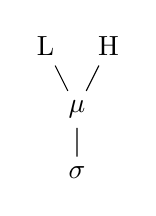
\begin{tikzpicture}
					\node (bt1) at (-.4,0.8) {L};
					\node (bt2) at (.4,0.8) {H};
					\node (bc1) at (0,0) {$\mu$};
					\node (bs1) at (0,-0.8) {$\sigma$};
					\draw (bt1) -- (bc1) -- (bs1);
					\draw (bt2) -- (bc1);
				\end{tikzpicture}
				\vspace{-0.5em}
				\subcaption{}
		\end{subfigure}} 
		
		\scalebox{0.7}{\begin{subfigure}[t]{1.5cm}			
				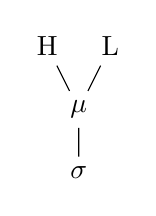
\begin{tikzpicture}
					\node (bt1) at (-.4,0.8) {H};
					\node (bt2) at (.4,0.8) {L};
					\node (bc1) at (0,0) {$\mu$};
					\node (bs1) at (0,-0.8) {$\sigma$};
					\draw (bt1) -- (bc1) -- (bs1);
					\draw (bt2) -- (bc1);
				\end{tikzpicture}
				\vspace{-0.5em}
				\subcaption{}
		\end{subfigure}} 
		
		\scalebox{0.7}{			\begin{subfigure}[t]{1.5cm}
				\centering 
				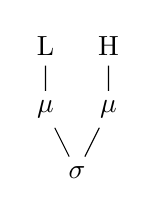
\begin{tikzpicture}
					\node (bt1) at (-.4,0.8) {L};
					\node (bt2) at (.4,0.8) {H};
					\node (bc1) at (-.4,0) {$\mu$};
					\node (bc2) at (.4,0) {$\mu$};
					\node (bs1) at (0,-0.8) {$\sigma$};
					\draw (bt1) -- (bc1) -- (bs1);
					\draw (bt2) -- (bc2) -- (bs1);
				\end{tikzpicture}
				\vspace{-0.5em}
				\subcaption{}
		\end{subfigure}} 
		%				\hspace{-1.3em}
		\scalebox{0.7}{			\begin{subfigure}[t]{1.6cm}
				\vspace{-4em}
				\centering				
				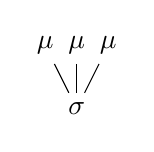
\begin{tikzpicture}
					\node (bc1) at (-.4,0) {$\mu$};
					\node (bc2) at (0,0) {$\mu$};
					\node (bc3) at (.4,0) {$\mu$};
					\node (bs1) at (0,-0.8) {$\sigma$};
					\draw (bc1) -- (bs1);
					\draw (bc2) -- (bs1);
					\draw (bc3) -- (bs1);
				\end{tikzpicture}
				\vspace{0.2em}
				\subcaption{}
		\end{subfigure}} 
		
		\scalebox{0.7}{	\begin{subfigure}[t]{1.6cm}
				\centering
				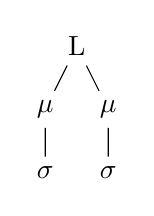
\begin{tikzpicture}
					\node (bt1) at (0,0.8) {L};
					% \node (bt2) at (.4,0.8) {L};
					\node (bc1) at (-.4,0) {$\mu$};
					\node (bc2) at (.4,0) {$\mu$};
					\node (bs1) at (-.4,-0.8) {$\sigma$};
					\node (bs2) at (0.4,-0.8) {$\sigma$};
					\draw (bt1) -- (bc1) -- (bs1);
					\draw (bt1) -- (bc2) -- (bs2);
				\end{tikzpicture}
				\vspace{-0.5em}
				\subcaption{}
		\end{subfigure}} 
		
		\scalebox{0.7}{			\begin{subfigure}[t]{2cm}
				\centering
				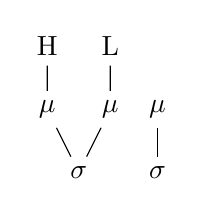
\begin{tikzpicture}
					\node (bt1) at (-.4,0.8) {H};
					\node (bt2) at (.4,0.8) {L};
					\node (bc1) at (-.4,0) {$\mu$};
					\node (bc3) at (1,0) {$\mu$};
					\node (bc2) at (.4,0) {$\mu$};
					\node (bs1) at (0,-0.8) {$\sigma$};
					\node (bs2) at (1,-0.8) {$\sigma$};
					\draw (bt1) -- (bc1) -- (bs1);
					\draw (bt2) -- (bc2) -- (bs1);
					\draw (bc3) -- (bs2);
				\end{tikzpicture}				\vspace{-.5em}
				\subcaption{}
		\end{subfigure}} \\ \hline
	\end{tabular} \caption{}
	\label{rules}
\end{table}

Among the constraints listed in Table x, the first three are hard constraints 
that define the basic phonology of the tone inventory and syllable weight. 
The remaining two are better described as violable constraints in \citet{zoll2003optimal} 
and related work. Newman also points out that there are exceptional words that violate 
these constraints. These constraints will serve as the \textit{baseline grammar}, 
which allows us to evaluate whether the learning algorithms meaningfully improve over a 
linguistically informed grammar. 

As for the empirical data, a curated corpus was constructed from the Hausa 
database \citep{wold-4} in the \textit{World Loanword Database} (WOLD, \citet{wold}). 
The curated corpus contains 621 monomorphemic, non-borrowed words from the core 
vocabulary, transcribed in orthography. These forms are converted into both 
string and AR representations, yielding 61 unique types. Table~X provides 
two examples of these representations. 

\begin{table}
	\begin{tabular}{c|c|c|c}
	\hline
Form & String & Feature & AR \\ \hline 
		\makecell{ \textit{mù.tûm} \\ `person'}	 & L.HL & \makecell{+L\\-C} .\makecell{-L\\-C}\makecell{+L\\-C}&
		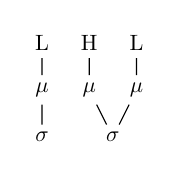
\begin{tikzpicture}
			[scale=0.6, every node/.style={scale=0.8}]
			\node (t0) at (1,1) {L};
			\node (t1) at (2,1) {H};
			\node (t2) at (3,1) {L};
			\node(c1) at (1,0) {$\mu$};
			\node(c2) at (2,0) {$\mu$};
			\node(c3) at (3,0) {$\mu$};
			\node (s1) at (1,-1) {$\sigma$};
			\node (s2) at (2.5,-1) {$\sigma$};
			\draw (t0) -- (c1) -- (s1);
			\draw (t1) -- (c2) -- (s2);
			\draw (t2) -- (c3) -- (s2);
		\end{tikzpicture} \\ \hline
 (nonce)	 & R.H &  \makecell{+L \\ +C} .\makecell{-L \\ -C}&
		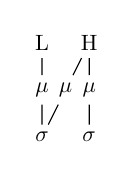
\begin{tikzpicture}
			[scale=0.6, every node/.style={scale=0.8}]
			\node (t0) at (1.5,1) {L};
			\node (t1) at (2.5,1) {H};
			\node(c1) at (1.5,0) {$\mu$};
			\node(c2) at (2,0) {$\mu$};
			\node(c3) at (2.5,0) {$\mu$};
			
			\node (s1) at (1.5,-1) {$\sigma$};
			\node (s2) at (2.5,-1) {$\sigma$};
			\draw (t0) -- (c1) -- (s1);
			\draw (t1) -- (c2) -- (s1);
			\draw (t1) -- (c3) -- (s2);
		\end{tikzpicture} \\ \hline
	\end{tabular}
	\caption{Positive and Negative forms in three representations}
	\label{tab.threereps}
\end{table}


For example, the word \textit{kòò.gíí} `river' is represented as \textit{LL.HH}, 
indicating that the word has two bimoraic syllables: the first associated with 
L and the second with H. The syllable boundary is indicated by a period. 
Contour tones are decomposed into level tones; thus, the falling tone in 
\textit{mù.tǔm} `person' is represented as \textit{HL}. Without assuming any prior 
tonal knowledge, we additionally introduce \textit{R} and \textit{F} into 
the alphabet to represent monosyllabic LH and falling HL tones, respectively.

For AR conversion, each form is analyzed as a three-tier structure: mora, syllable, 
and tone. Again, the OCP is assumed, and contour tones are decomposed into level units. 
One difference from the string representation is that AR does not need to expand its 
tonal inventory to include R and F, since contours are analyzed as multiple tones 
associating with a single TBU. Additionally, since syllable boundaries are naturally 
reflected in the AR structure, we do not need a separate marker for syllable boundaries.
In the actual implementation, the AR is encoded as a pair of adjacency matrices, which we 
do not discuss in further detail here.



In total, the experiment therefore compares the following five conditions:


\begin{table}[h]
	\centering
	\begin{tabular}{lll}
		\hline
		\textbf{Condition} & \textbf{Model} & \textbf{Representation} \\
		\hline
		Base-Str& Baseline & String \\
		Base-AR     & Baseline & AR \\
		\textsc{BUFIA}-Str & \textsc{BUFIA} & String \\
		\textsc{BUFIA}-AR     & \textsc{BUFIA} & AR \\
		\textsc{MaxEnt}-Str & \textsc{MaxEnt} & String \\
		\hline
	\end{tabular}
	\caption{Experimental conditions comparing learning models and representational formats.}
	\label{tab:conditions}
\end{table}




\subsection{Evaluation}
We conducted a $4$-fold cross-validation procedure, partitioning the dataset 
into four equally sized folds. In each iteration, three folds are used for 
training and the remaining fold serves as the evaluation set. This process 
is repeated four times, with each fold acting as the test set once.

During evaluation, we do not test only on the held-out positive data. 
Instead, we construct two types of test sets: the \textit{regular set} and 
the \textit{extended set}.

The \textit{regular set} consists of the held-out positive forms (16 types) 
together with an equal number of manually constructed negative forms. 
Each constructed negative form violates at least one of the baseline 
constraints. For each condition, the test items are encoded in the 
corresponding representation (string or AR) and evaluated together with 
the positive data. This design allows us to assess whether the learned 
grammar over generates beyond the attested patterns.

The \textit{extended set} builds on the regular set by adding four 
exceptional positive types and four matched negative forms (40 in total). 
The exceptional forms are drawn from Hausa data 
reported by Newman and violate both \textsc{*Clash} and 
\textsc{*Nonfinal-Fall}. Newman notes that a few such forms do occur in the 
corpus and suggests that they may have historical explanations, although 
their precise source remains unclear. 

In model evaluation, a well-formedness judgment is counted as correct if the 
model accepts positive examples (whether from the held-out fold or the 
exceptional set) and rejects the negative examples. Performance is 
measured in terms of recall, precision, and F1 score over these 
classifications.

It should be noted that the \textsc{MaxEnt} model returns a gradient 
grammar in which all constraints are violable and assigned weights. 
However, for comparability with the categorical models, we 
convert the learned  \textsc{MaxEnt}  grammar into a categorical 
interpretation: candidate forms whose total weighted violation score 
is zero are treated as well-formed, whereas those with a non-zero 
weighted sum are treated as ill-formed. In other words, a test candidate 
is classified as well-formed only if it does not violate any constraint 
in the grammar.


\section{Results}
The averaged results across folds are shown in Tables~4 and~5. For both test sets, all models under both representational formats achieved perfect precision (1.000). This indicates that, regardless of the learning mechanism, both string and AR representations successfully reject the constructed ill-formed structures.

First, a comparison between baseline-str and baseline-ar shows that their results are identical. When the same grammar is applied to the two representations, it produces exactly the same predictions on the dataset. A closer inspection of the errors confirms that they are identical as well. This indicates that, when there is a one-to-one correspondence between representations, representational format alone does not affect the behavior of a fixed grammar over surface forms. It should be noted, however, that we explicitly ensured a one-to-one mapping between string and AR representations: no two forms in one system collapse into a single form in the other. In addition, the alphabets of the two representations differ. The string alphabet includes R, F, and explicit syllable boundary markers, whereas the AR representation includes mora and syllable tiers.

In contrast to the baseline grammar, recall and F1 scores for the learned grammars show greater variation. Across both test sets, the same performance pattern emerges

This ranking is consistent across both the held-out data and the extended test set including exceptional forms.

Comparing the two versions of the BUFIA learner, the choice of representation clearly affects learning outcomes. Specifically, \textsc{BUFIA-string} achieves an F1 score of 0.950 on the regular test set and 0.903 on the extended test set. When switching to AR representations, the F1 score increases to 0.984 on the regular set and 0.968 on the extended set. With the learning algorithm held constant, this improvement indicates that AR representations yield more accurate predictions for unseen attested forms.

Finally, we evaluated MaxEnt-string. Its learning performance is lower than that of all other models, including the baseline grammar.

\begin{table*}
	\centering
	\begin{tabular}{l|ccc|ccc}
		\hline
		& \multicolumn{3}{|c|}{\textbf{Test Set 1}} & \multicolumn{3}{c}{\textbf{Test Set 2}} \\
		\hline
		\textbf{Model} 
		& \textbf{Recall} & \textbf{Prec.} & \textbf{F1}
		& \textbf{Recall} & \textbf{Prec.} & \textbf{F1} \\
		\hline
		baseline-str & 0.813 & 1.000 & 0.894 & 0.650 & 1.000 & 0.786 \\
		baseline-ar & 0.813 & 1.000 & 0.894 & 0.650 & 1.000 & 0.786 \\
		bufia-str    & 0.906 & 1.000 & 0.950 & 0.825 & 1.000 & 0.903 \\
		MaxEnt-str   & 0.641 & 1.000 & 0.774 & 0.525 & 1.000 & 0.680 \\
		bufia-ar     & 0.984 & 1.000 & 0.992 & 0.938 & 1.000 & 0.968 \\
		\hline
	\end{tabular}
	\caption{Averaged performance across four folds on Test Set 1 (16 held-out positives + 16 negatives) and Test Set 2 (20 positives, including rare forms, + 20 negatives). All models achieve perfect precision; differences reflect recall and F1.}
	\label{tab:results-merged}
\end{table*}

\section{Discussion}
Recall the questions posed earlier: first, can tonotactics be learned directly over ARs? 
If so, what differences in learning outcomes emerge between AR and string representations?

The results show that the two representations do not differ in the baseline grammar, 
indicating that representational format alone does not change the behavior of a fixed 
grammar. Two points should be noted. First, the two representations are in bijective 
correspondence: each string representation has a unique AR counterpart. Under this 
one-to-one mapping, no learning differences arise at the baseline level. However, 
achieving this mapping requires the string representation to adopt a larger alphabet to 
encode combinations that are structurally explicit in ARs. In languages with monosyllabic 
contours or more complex tonal configurations, this requirement would further expand the 
alphabet. Second, this study focuses on surface phonotactics, but learning tonal 
processes more generally depends on changes in association rather than feature values. 
While these differences may be masked at the surface level, such structural changes are 
more naturally captured in ARs.

In contrast, when examining the computationally learned grammars, clear differences 
emerge across representational choices and learning models. Comparing the two BUFIA 
learners shows that learning over ARs achieves higher accuracy on attested forms without 
increased overgeneralization. This pattern remains robust even when the dataset includes 
rare forms that violate previously established constraints, suggesting that learning 
benefits from structurally informed representations.

The relatively low performance of the MaxEnt model may raise questions. One possible explanation is the limited dataset size, which contains fewer than 70 unique types. However, two considerations are relevant. First, under a string representation, the complete alphabet and its combinatorial space remain substantially smaller than the feature spaces typical of segmental phonology. Second, we use type-based rather than token-based data. This is unlikely to be a major limitation because Hausa tonal patterns are highly skewed and approximately Zipfian: a majority of forms share the same tonal structures. Even with larger datasets including frequency information, the impact on MaxEnt performance may be limited, particularly when constraints behave effectively as categorical restrictions.

\section{Conclusion}
This paper compares the tonotactic learning outcomes over string and ARs by examining the 
outputs of two versions of BUFIA on the same Hausa data. Results show that learning over 
ARs captures tonal generalizations more efficiently than strings, which fails to capture 
structural information at the sub-syllabic level. Future research will more precisely 
study the effects of the learner's traversal of the space, different `feature' 
specifications for string representations, and the role of word boundaries. More 
generally, this paper advocates for the use of interpretable learning models to help 
distinguish between different theories of linguistic representation.


\bibliography{refs.bib}


\end{document}
